\documentclass[12pt]{article}

\usepackage[a4paper, margin=1in]{geometry}
\usepackage{xcolor}
\usepackage{amsmath}
\usepackage{amssymb}
\usepackage{tcolorbox}
\usepackage{fontawesome5} % icons
\usepackage{hyperref}
\usepackage{graphicx}
\usepackage{float}
\usepackage{comment}
\usepackage[nameinlink,capitalize,noabbrev]{cleveref}
\usepackage{subcaption} % modern replacement for the deprecated subfigure package
\usepackage{tikz}
\usetikzlibrary{arrows.meta,positioning,shapes.geometric}
\usepackage{listings}
\usepackage{booktabs}
\usepackage{array}

\setlength{\parindent}{0pt}

% --- COLOR PALETTE (same as other TAI materials) ---
\definecolor{maincolor}{HTML}{2A9D8F} % teal
\definecolor{accentcolor}{HTML}{E76F51} % orange
\definecolor{lightcolor}{HTML}{FFDEAD}
\definecolor{darkcolor}{HTML}{264653}

% Tell cleveref how to name the counters
\crefname{exercise}{assignment}{assignments}
\Crefname{exercise}{Assignment}{Assignments}

% --- ASSIGNMENT STYLE ---
\newcounter{exercise}

% Optional label: \exercisetitle[<label>]{<Title>}
\newcommand{\exercisetitle}[2][]{%
  \refstepcounter{exercise}%
  \vspace{0.5cm}%
  \colorbox{maincolor}{%
    \makebox[\dimexpr\linewidth-2\fboxsep][l]{%
      \textcolor{white}{\faPen\ Assignment \theexercise:~ #2}%
    }%
  }%
  \if\relax\detokenize{#1}\relax\else\label{#1}\fi
  \vspace{0.3cm}%
}

% --- STEP HEADER (phase divider inside the handout) ---
\newcommand{\steplabel}[2]{%
  \vspace{0.7cm}%
  \noindent\textcolor{darkcolor}{\rule{\linewidth}{0.8pt}}\\[2pt]
  {\large\textcolor{darkcolor}{\textbf{#1}}}\hfill\textcolor{gray}{\faClock\ #2}\\[2pt]
  \noindent\textcolor{darkcolor}{\rule{\linewidth}{0.4pt}}
  \vspace{0.2cm}%
}

% --- IMPORTANT BOX ---
\newtcolorbox{importantbox}{
  colback=lightcolor,
  colframe=accentcolor,
  arc=4mm,
  boxrule=1pt,
  left=6pt,
  right=6pt,
  top=6pt,
  bottom=6pt
}

% --- PROMPT BOX ---
\newtcolorbox{promptbox}{
  colback=white,
  colframe=maincolor,
  arc=4mm,
  boxrule=1pt,
  left=6pt,
  right=6pt,
  top=6pt,
  bottom=6pt
}

% --- QUESTION BOX (with starred variant and cleveref names) ---
\crefname{question}{question}{questions}
\Crefname{question}{Question}{Questions}

\makeatletter
\newcounter{question}
\newlength\questionheight
\setlength\questionheight{4cm} % default answer box height

% \question{<text>}                  -> with TextField (default height)
% \question[<height>]{<text>}        -> with TextField (custom height)
% \question*{<text>}                 -> no TextField, still numbered
\newcommand{\question}{\@ifstar{\question@text}{\question@field}}

\newcommand{\question@heading}[1]{%
  \refstepcounter{question}%
  \vspace{0.3cm}%
  \noindent\textbf{\faEdit\ Question \thequestion: #1}%\\[0.3em]%
}

\newcommand{\question@text}[1]{%
  \question@heading{#1}%
}

\newcommand{\question@field}[2][\questionheight]{%
  \question@heading{#2}%
 \\[0.3em] \begin{Form}
    \TextField[
      name=Q\thequestion,
      multiline=true,
      width=\linewidth,
      height=#1,
      charsize=10pt,
      bordercolor={0 0 0},
      borderwidth=1.8,
      backgroundcolor={1 1 1}
    ]{}
  \end{Form}
  \vspace{0.3cm}%
}
\makeatother

% --- SOLUTION BOX ---
% --- Teacher toggle ---
\newif\ifteacher
\teacherfalse % Write teacherfalse for the student version, teachertrue for the teacher version

% --- Solution environment ---
\newtcolorbox{solutionbox}{colback=gray!10,colframe=black!60!black,arc=1mm,boxrule=1pt}

\ifteacher
\newenvironment{solution}{%
  \begin{solutionbox}\textbf{\faChalkboardTeacher\ Solution / notes for the teacher:}
}{%
  \end{solutionbox}
}
\else
  \excludecomment{solution}
\fi

% --- CODE LISTING STYLE ---
\lstdefinestyle{micropython}{
  basicstyle=\ttfamily\small,
  keywordstyle=\color{maincolor}\bfseries,
  commentstyle=\color{gray},
  stringstyle=\color{accentcolor},
  numbers=left,
  numberstyle=\tiny\color{gray},
  breaklines=true,
  frame=single,
  rulecolor=\color{darkcolor!40},
  backgroundcolor=\color{gray!5},
  showstringspaces=false,
  language=Python
}

% --- GRIDWORLD TIKZ HELPER ---
% state = row*3 + col ; row 0 is the TOP row (matches the microbit code)
\newcommand{\gridcell}[3]{% row, col, content
  \node at (#2+0.5, 2.5-#1) {#3};
}
\newcommand{\gridworld}[1]{%
  \begin{tikzpicture}[scale=1.15]
    \draw[step=1cm, darkcolor, thick] (0,0) grid (3,3);
    \foreach \r in {0,1,2}{
      \foreach \c in {0,1,2}{
        \pgfmathtruncatemacro{\st}{\r*3+\c}
        \node[gray,font=\tiny] at (\c+0.15, 2.85-\r) {\st};
      }
    }
    #1
  \end{tikzpicture}%
}

\begin{document}

\begin{titlepage}

\vspace*{1cm}

% --- Project logo ---
\begin{center}
    
\includegraphics[height=3cm]{Figures/Logo_TAI_Transparent.png}
\end{center}

\vspace{0.8cm}

\begin{center}
    {\Huge \bfseries \color{maincolor} A rover learning on an exoplanet\par}
    \vspace{0.5cm}

    {\Large \color{accentcolor} Teaching with AI (TAI) \par}

    \vspace{1.5cm}

    \begin{center}
{\large
Mirte van der Eyden$^{1}$, Andrea L\'{o}pez Incera$^{2}$, Georgios Errikos Hlapanis$^{3}$ \\[0.3cm]

{\small
$^{1}$ Institut f\"{u}r Fachdidaktik, Universit\"{a}t Innsbruck \\
mirte.van-der-eyden@uibk.ac.at \\[0.2cm]

$^{2}$ Departament de did\`{a}ctica de la matem\`{a}tica i les ci\`{e}ncies experimentals, Universitat Aut\`{o}noma de Barcelona \\
andrea.lopez.incera@uab.cat \\[0.2cm]

$^{3}$ 2nd Lyceum of Kos, University of the Aegean \\
hlapanis@2lykko.gr, hlapanis@aegean.gr
}
}
\end{center}

\end{center}

\vfill

% --- Logos at the bottom ---
\begin{center}
\begin{tabular}{cccc}

\includegraphics[height=1.5cm]{Figures/Logos/universitaet-innsbruck-logo-cmyk-farbe.jpg} &

\includegraphics[height=1.5cm]{Figures/Logos/logotipuab-v1-verd.png} &

\includegraphics[height=1.5cm]{Figures/Logos/EN Co-funded by the EU_POS.jpg} \\

\includegraphics[height=1.5cm]{Figures/Logos/IMG_1189.PNG} &

\includegraphics[height=1.8cm] {Figures/Logos/2nd Lyceum of Kos logo.jpg} &

\includegraphics[height=1.5cm]{Figures/Logos/NEXT_prov_logo.png}
\end{tabular}
\end{center}

\vspace{0.5cm}

\begin{center}
    {\small Project funded by Erasmus+ Programme of the European Union}
\end{center}

\end{titlepage}

% --- Description of activity ---
\vspace*{0.25\textheight}

Subject: Robotics and programming (age 16)

\vspace{0.3cm}

Activity duration: 2h 15min

\vspace{0.5cm}

Steps:
\begin{enumerate}
    \item Introduction: what is a rover, and how could it learn? (10 min)
    \item Meet the micro:bit: first MicroPython program (10 min)
    \item Assignment 1 -- Calibrate the rover: forward, turn, square (30 min)
    \item Introduction to reinforcement learning: environment, task, ingredients (10 min)
    \item Human simulation of learning, in pairs (20 min)
    \item The teacher explains the learning rule with a worked example (10 min)
    \item Assignment 2a -- Write the pseudocode of one round of learning (10 min)
    \item Assignment 2b -- Read the LLM-generated code and run it on the micro:bit (15 min)
    \item Assignment 3 -- Final demonstration: the cutebot learns on the grid (20 min)
\end{enumerate}

Learning goals:

\begin{itemize}
    \item Practice programming with the help of an LLM (prompt engineering).
    \item Learn to read and understand MicroPython code written by an LLM.
    \item Understand the basic ingredients of reinforcement learning (state, action, reward, Q-value) and the Q-learning update rule.
    \item Apply the above to program and observe a rover learning a simple navigation task.
\end{itemize}

Materials needed (per group of 2-4 students): 1 micro:bit V2 + USB cable, 1 ELECFREAKS Cutebot + battery pack, 1 laptop with access to \url{python.microbit.org} and an LLM (e.g. ChatGPT or Gemini), 1 printed 3x3 grid (template in \cref{app:grid}, cells at least 15 cm wide so the cutebot's movement is clearly visible).

\newpage

% --- HEADER / BRANDING ---
\begin{center}
    {\LARGE \color{maincolor} A rover learning on an exoplanet}\\[5pt]
    {\large \textit{A robotics and reinforcement learning lesson with AI}}\\
    \rule{\linewidth}{1pt}
\end{center}

\vspace{0.5cm}

\begin{importantbox}
\textbf{The challenge:} A rover has just landed on an exoplanet and must travel between two research stations to keep them supplied. The round trip to Earth for a radio signal takes so long that remote control is impossible: the rover has to learn, by itself, which way to go. As a team of engineers, your job today is to build that rover's brain -- first teaching it to move, and then teaching it to \emph{learn}.
\end{importantbox}

\steplabel{Step 1. What is a rover, and how could it learn?}{10 min}

\textcolor{accentcolor}{\textbf{\faLightbulb\ Initial ideas}}

\vspace{0.2cm}
% Placeholder: AI-generated hero image of a small rover exploring a rocky exoplanet surface.
% \begin{figure}[H]\centering
% \includegraphics[width=0.6\linewidth]{Figures/rover_exoplanet_hero.png}
% \caption{AI-generated concept art: a rover exploring an exoplanet. \emph{(placeholder -- to be generated)}}
% \end{figure}

\question{What do you think a rover is? What is it used for?}

\question{Have you ever seen a robotic vacuum cleaner at home? What do you think it has in common with a rover on another planet?}

\begin{solution}
Guide the discussion towards: both are autonomous mobile robots that must operate without a human directly steering them at every instant. A robot vacuum does not know your house's floor plan when you buy it -- it bumps into things, senses its surroundings, and gradually finds a more efficient way to cover the room. A planetary rover faces the same problem, but on a much bigger and more dangerous scale, and with a huge communication delay to Earth. The core idea of the lesson is: \emph{if a rover cannot be told exactly what to do at every step, it needs a way to try, fail, and improve on its own.} That is what today's lesson is about.
\end{solution}

\question{Very generally, what do you think any autonomous robot (rover, vacuum cleaner, self-driving car\ldots) needs in order to move around and act on its own?}

\begin{solution}
Three big ingredients, which map directly onto the hardware used today: \textbf{input} (sensors, to perceive the environment), \textbf{processing} (a ``brain'' that decides what to do), and \textbf{output} (motors, to act on the world). Today the micro:bit will be the brain and the cutebot will be the muscles.
\end{solution}

\vspace{0.4cm}
\steplabel{Step 2. Meet the micro:bit}{10 min}

The \textbf{micro:bit V2} will be the brain of your rover. It is a tiny computer with a $5\times5$ grid of LEDs, two buttons, and several sensors. You will program it in \textbf{MicroPython}, a version of Python designed for small devices, using the online editor at \url{python.microbit.org}. You do not need to be a Python expert: today, an LLM (ChatGPT, Gemini, or similar) will be your \textbf{co-pilot}. Your job is not to memorize syntax, but to describe clearly what you want the code to do.

% Placeholder / real photo: micro:bit V2 board.
% Suggested source if using a real photo (cite in the caption): microbit.org
% \begin{figure}[H]\centering
% \includegraphics[width=0.45\linewidth]{Figures/microbit_v2.png}
% \caption{The micro:bit V2. Source: microbit.org \emph{(placeholder)}}
% \end{figure}

\begin{promptbox}
\textbf{Try it:} Connect your micro:bit to the laptop with the USB cable, open \url{python.microbit.org}, and ask your AI co-pilot:\\[4pt]
\textit{``Write a simple MicroPython program for a micro:bit that shows a smiley face on the LED display.''}\\[4pt]
Paste the code into the editor, click \textbf{Send to micro:bit}, and check that it works!
\end{promptbox}

%question{Look at the code the AI gave you. Can you find the part that controls which LEDs turn on? What do you think would happen if you asked the AI to make the face blink, or to show a different image?}

%\begin{solution}
%Most AI answers will use \texttt{display.show(Image.HAPPY)} or a manually built \texttt{Image("...")} string of 25 digits (one per LED, 0-9 brightness). Blinking usually adds a \texttt{while True} loop with \texttt{display.clear()} and \texttt{sleep()} calls. This is a good moment to point out that the AI already used a \texttt{while True} loop and \texttt{sleep()} -- both will reappear in the rover code later.
%\end{solution}

\exercisetitle{Calibrate your rover}\label{ass:calibrate}
\textcolor{gray}{\faClock\ 30 min}

\textcolor{accentcolor}{\textbf{\faLightbulb\ Constructing new ideas}}

\vspace{0.2cm}
If the micro:bit is the brain, the \textbf{ELECFREAKS Cutebot} is the muscle that will carry it across the exoplanet with its two independent wheel motors. Slot the micro:bit into the top of the cutebot and make sure the battery pack is connected and switched on.

% Placeholder / real photo: Cutebot chassis.
% Suggested source if using a real photo (cite in the caption): thepihut.com
% \begin{figure}[H]\centering
% \includegraphics[width=0.45\linewidth]{Figures/cutebot.png}
% \caption{The ELECFREAKS Cutebot. Source: thepihut.com \emph{(placeholder)}}
% \end{figure}

\begin{importantbox}
\textbf{The golden prompting rule:} Always start your prompt with \textit{``I am programming an ELECFREAKS Cutebot with a micro:bit, using MicroPython and the \texttt{Cutebot} library.''} This helps the AI use the correct commands. Also give the AI the file \texttt{Cutebot.py} (already loaded in your editor) so it knows which functions are available, e.g. \texttt{ct.set\_motors\_speed(left\_speed, right\_speed)}, with speeds from $-100$ to $100$.
\end{importantbox}

Place your rover on \textbf{cell 0} of your printed grid (top-left corner, facing right/East) for every task below.

\vspace{0.3cm}
\textbf{\faArrowRight\ Task 1: Drive in a straight line}

\begin{itemize}
  \item[$\square$] Ask the AI: \textit{``Write a script to make the cutebot drive straight forward for a short time, then stop.''}
  \item[$\square$] Does it veer left or right? Ask the AI how to compensate by giving the two wheels slightly different speeds.
  \item[$\square$] Tune the driving time so the rover moves \textbf{exactly one grid cell} and stops.
\end{itemize}

\question{Write down your final values for the speed and the driving time (in ms) it takes your rover to cross exactly one cell. You will need these numbers later!}

\vspace{0.3cm}
\textbf{\faSync\ Task 2: Turn 90 degrees}

\begin{itemize}
  \item[$\square$] Ask the AI: \textit{``Write a script to make the cutebot turn right on the spot for a short time, then stop.''}
  \item[$\square$] Adjust the turning time until the rover rotates \textbf{exactly a quarter turn} (90\textdegree).
\end{itemize}

\question{What is your turn time in milliseconds for a perfect 90\textdegree\ turn?}

\vspace{0.3cm}
\textbf{\faVectorSquare\ Task 3: Walk a square}

\begin{itemize}
  \item[$\square$] Combine Tasks 1 and 2: ask the AI to use a loop that repeats (drive forward, turn 90\textdegree) four times.
  \item[$\square$] Try it on your printed grid: the rover should trace a perfect square of 4 cells and end up exactly where it started, facing the same direction.
  \item[$\square$] Keep fine-tuning speed and timings until it lands back on the start cell.
\end{itemize}

\question{Did your rover end up back on the exact starting cell, facing the same way? If not, what did you change to fix it?}

\begin{solution}
There is no single ``correct'' value: it depends on battery level, floor friction, and the individual motors, which is exactly the point of calibration. Typical starting values used in the demonstration code are speed $=30$ (out of 100), \texttt{MOVE\_TIME} $\approx 200$~ms per cell, \texttt{TURN\_TIME} $\approx 350$~ms per 90\textdegree\ turn -- but every rover is different! If students get stuck, the reference solution below can be given as a safety net (do not hand it out immediately -- guide them to reach it through their own prompting first).

\begin{lstlisting}[style=micropython]
from microbit import *
from Cutebot import *

ct = CUTEBOT()
SPEED = 30
MOVE_TIME = 200   # ms to cross one grid cell
TURN_TIME = 350   # ms for a 90-degree turn

def forward():
    ct.set_motors_speed(SPEED, SPEED)
    sleep(MOVE_TIME)
    ct.set_motors_speed(0, 0)

def turn_right():
    ct.set_motors_speed(SPEED, -SPEED)
    sleep(TURN_TIME)
    ct.set_motors_speed(0, 0)

# Walk a square:
for i in range(4):
    forward()
    turn_right()
\end{lstlisting}
This same file is provided as \texttt{01\_forward.py}, \texttt{02\_turn90.py} and \texttt{03\_square.py} in the \textit{Student Materials} folder, to be used only if a group is completely stuck.
\end{solution}

\steplabel{Step 3. Introduction to reinforcement learning}{10 min}

\textcolor{accentcolor}{\textbf{\faLightbulb\ Initial ideas}}

Now that your rover can move, it is time to teach it to find its own way. From now on, the rover will live inside a simplified world: a \textbf{3$\times$3 grid}, printed on paper, with 9 possible cells (\emph{states}). The rover starts at cell 0 (top-left) and its task is to reach cell 8 (bottom-right, the research station) in as few moves as possible.

\begin{figure}[H]
\centering
\gridworld{
  \node[circle,fill=maincolor!35,minimum size=0.7cm] at (0.5,2.5) {\faRobot};
  \node[circle,fill=accentcolor!45,minimum size=0.7cm] at (2.5,0.5) {\faFlagCheckered};
}
\caption{The 3$\times$3 gridworld. The rover (\faRobot) starts at state 0, the goal (\faFlagCheckered) is state 8. Small grey numbers label the 9 states.}
\end{figure}

At every cell, the rover can choose one of four \textbf{actions}: move up, down, left or right (if an action would push it off the grid, it simply stays in place).

\question*{This is the kind of learning problem called \emph{reinforcement learning} (RL): the rover is not told the correct path in advance. Based on everything we said in Step 1, what information do you think the rover needs to be able to learn the shortest path by trial and error? Think about what it must perceive, what it must remember, and what tells it whether it is doing well or badly.}

\begin{solution}
After students think about it and express their ideas, in a consensus, guide students towards three ingredients, which the teacher can then name explicitly:
\begin{itemize}
  \item \textbf{Input / state}: the rover must know which cell it is currently in.
  \item \textbf{Memory}: the rover must remember, for every state and every possible action, some measure of ``how good'' that action has been so far. This is the \textbf{Q-value}: $Q(s,a)$, one number for every state-action pair. With 9 states and 4 actions, that is a table of $9\times4=36$ numbers -- the rover's entire ``memory'' of what it has learned.
  \item \textbf{Reward}: a signal that tells the rover, after each move, whether that move was good or bad, so it can update its memory.
\end{itemize}
\end{solution}

\vspace{0.4cm}
\steplabel{Step 4. Human simulation: learning in pairs}{20 min}

\textcolor{accentcolor}{\textbf{\faLightbulb\ Constructing new ideas}}

Before the rover learns, \emph{you} will. Work in pairs on your printed grid.

\begin{importantbox}
\begin{itemize}
  \item One student is the \textbf{Rover}: close your eyes (or turn away from the grid). You do not know the grid layout, nor where the reward is. You can only call out one action at a time: ``up'', ``down'', ``left'' or ``right''.
  \item The other student is the \textbf{Environment}: select a cell to put the reward (the Rover cannot see it). Watch the grid and, after every move the Rover calls out:
   \begin{itemize}
    \item Tell it the cell number where it landed (state)
    \item Give it feedback (reward) using this reward scheme (matching exactly what the microbit code will use later):
    \end{itemize} 
\end{itemize}

\begin{center}
\renewcommand{\arraystretch}{1.3}
\begin{tabular}{|l|c|}
\hline
\textbf{What happened} & \textbf{Reward} \\
\hline
Normal move (moved to a new, valid cell) & $-1$ \\
\hline
Tried to move off the grid (stays in place) & $-5$ \\
\hline
Reached the goal cell (state 8) & $+10$ \\
\hline
\end{tabular}
\end{center}
\end{importantbox}

Play a few rounds, swapping roles. Each full attempt (from the start cell until reaching the goal) is called an \textbf{episode}. After a few rounds, the Rover can open their eyes and see where the reward was, and the Environment can tell which was the shortest path.

\question{Rover, was it easier to find the goal in your second or third attempt than in your first? Why?}

\begin{solution}
Yes -- this is the whole point of the activity. Even without seeing the grid, the ``Rover'' student starts to remember which moves led to good or bad feedback (e.g. ``going right from the corner got me a -5, so I shouldn't do that again''). That is exactly the intuition behind updating Q-values: use past experience (rewards) to make better decisions in the future.
\end{solution}

\question{Rover, what were you memorizing to be able to learn the path to the reward?}

\begin{solution}
This answer is of course open, since humans have different strategies to remember things, but the most basic thing that one needs to remember is: which action to take at which state.
\end{solution}

\question{Rover, did you always take the same action from the same cell, or did you sometimes try something new on purpose? Why might ``trying something new'' be useful, even if you already found something that works?}

\begin{solution}
This introduces the \textbf{explore vs. exploit} trade-off. Always repeating the first thing that worked (\emph{exploit}) can lock the rover into a path that works but is not the shortest. Occasionally trying a random action (\emph{explore}) lets the rover discover better paths it would otherwise never try. In the code, this is controlled by the parameter \texttt{epsilon} ($\varepsilon$): with probability $\varepsilon$ the rover picks a random action; otherwise, it picks the action it currently believes is best.
\end{solution}

\question{How do you think the actual rover remembers where to go, based on the environment giving it a reward when it reaches the goal?}

\vspace{0.4cm}
\steplabel{Step 5. The learning rule: Q-learning}{10 min}

\textcolor{accentcolor}{\textbf{\faLightbulb\ Explaining the idea}} \textit{(teacher-led)}

The algorithm the rover uses is called \textbf{Q-learning}. The rover keeps a table $Q(s,a)$: one number for every (state, action) pair, representing how good it currently believes that action $a$ is for that state $s$. The higher the Q value is for an action (at a given state), the better that action is. 

The Q table is the rover's memory. At the start, the rover knows nothing, so every entry is $Q(s,a)=0$.

After every move, the rover updates its estimate using the reward it just received. A first, simplified version of the rule would be:
\[
Q(s,a) \;\leftarrow\; Q(s,a) \;+\; \alpha\Big[\, r \;-\; Q(s,a) \,\Big]
\]
where $r$ is the reward just received and $\alpha$ (the \textbf{learning rate}, between 0 and 1) controls how much the new information overwrites the old estimate. But this only looks at the \emph{immediate} reward -- it does not think ahead. The full Q-learning rule also considers how promising the \emph{next} state looks:
\[
Q(s,a) \;\leftarrow\; Q(s,a) \;+\; \alpha\Big[\, r \;+\; \gamma \max_{a'} Q(s',a') \;-\; Q(s,a) \,\Big]
\]
where $s'$ is the state the rover ends up in, $\max_{a'} Q(s',a')$ is the best Q-value available from that next state (``how good does the future look from here''), and $\gamma$ (\textbf{discount factor}, between 0 and 1) controls how much the rover cares about future rewards versus immediate ones.

\begin{importantbox}
The arrow $\leftarrow$ means that the value to its left $Q(s,a)$ changes to a new value, which is the result of the operation to its right.
\end{importantbox}

\begin{promptbox}
\textbf{A fully worked example of the rover's first decision and move.} Suppose $\alpha = 0.5$, $\gamma = 0.9$, and every $Q$-value still equals 0 (the rover has not learned anything yet). The rover is at state 0 and, by exploring, randomly chooses the action \textbf{right}.
\begin{enumerate}
  \item It moves to state 1 (a normal, valid move), so the reward is $r = -1$.
  \item Its old estimate was $Q(0,\text{right}) = 0$.
  \item The best value available from the new state ($s=1$) is $\max_{a'} Q(1,a') = 0$ (still nothing learned there, so all Q values are zero).
  \item Update the old estimate $Q(0,\text{right}) = 0$ to: \\
  $Q(0,\text{right}) \leftarrow 0 + 0.5 \times \big[-1 + 0.9\times 0 - 0\big] = 0.5\times(-1) = \mathbf{-0.5}$
\end{enumerate}
The rover now remembers that, from state 0, going right was slightly disappointing. Over many episodes, these small updates accumulate: cells and actions that lead (even indirectly) to the goal end up with high Q-values, and the direct penalty of $-5$ for driving off the grid quickly teaches the rover to avoid the edges.
\end{promptbox}

\begin{importantbox}
\textbf{How the rover chooses an action:} With some probability (that you choose as a programmer), the rover picks an action randomly from its options: \{up, down, left, right\}. Otherwise, it picks the action with the highest Q value. This is like saying, `I roll a die, and if it is a 6 (low probability), I pick a random action; but if it is any other value from 1 to 5 (high probability), I choose the action with highest Q value'.
\end{importantbox}


\question{Work out an example yourself, following the same steps as in the example above, to convince yourself that this works. Imagine that it is *the first time* the rover gets to the reward (cell 8). It is in cell 5 and moves down to cell 8. What would be the updated value of $Q(5,\text{down})$? On the \emph{next} episode, how could that reward $+10$ ``travel backwards'' to help the rover in the cell next to the one just before the goal (for example, if in next episode, the rover gets to cell 2, how does it increase the Q value of going down to cell 5)?}

\begin{solution}
The very last action taken, the one that lands the rover on state 8, gets its $Q$-value pushed up directly by the $+10$ reward: $Q(5,\text{down}) \leftarrow 0 + 0.5 \times \big[10 + 0.9\times 0 - 0\big] = 0.5\times(10) = \mathbf{5}$.

On a later episode, when the rover is in the cell \emph{next to} the one before the goal and considers moving towards it, the $\gamma \max_{a'}Q(s',a')$ term will now be large (because that neighbouring state already has a high Q-value from the previous episode), so that action's Q-value increases too -- even though the reward for that particular move was only $-1$. This is how the reward from the goal gradually ``propagates backwards'' across the grid over many episodes, until the whole shortest path is reflected in the Q-table.
\end{solution}

\textcolor{maincolor}{\textbf{\faPen\ Watch the Q values grow throughout the learning process.}} Open the Google collab notebook `RL\_Rover\_Qvalues\_Simulation.ipynb' provided as additional material. Run all cells and choose from the points below what to do.

\begin{itemize}
  \item Basic $\rightarrow$ Go to point 3, where you see pictures at different moments of the learning process of the highest Q value for each grid cell. You can also select which episode to see by dragging a slider. 
  \item Advanced $\rightarrow$ Check the rest of the points, where you can see in different ways how the Q values grow, and how the rover learns.
  \item At the end of the notebook, there is a simulation where you watch it evolve.
\end{itemize}





\exercisetitle{Program the rover's brain}\label{ass:pseudocode}
\textcolor{gray}{\faClock\ 25 min (10 + 15)}

\vspace{0.2cm}
\textbf{Part A -- Write the pseudocode} \textcolor{gray}{\faClock\ 10 min}

\question[6cm]{Based on everything discussed in Steps 3-5, write the \textbf{pseudocode} (step-by-step recipe, in your own words or simple diagrams -- no need for real code yet) of \emph{one single round} of interaction between the rover and the grid environment: from the moment it is in some state, to the moment its Q-table has been updated. Think about the steps you were doing in *one interaction* Rover-Environment (one decision + one movement) when you were the Rover and the Environment yourselves.}

\begin{solution}
There is more than one valid way to phrase this; the key steps to look for are:
\begin{enumerate}
  \item \textbf{Get} the current state $s$ (which cell the rover is in).
  \item \textbf{Choose} an action $a$: with probability $\varepsilon$ pick a random action (\emph{explore}); otherwise pick the action with the highest $Q(s,a)$ (\emph{exploit}).
  \item \textbf{Perform} the action (move the rover / update its position).
  \item \textbf{Observe} the new state $s'$ and the reward $r$.
  \item \textbf{Learn}: update $Q(s,a)$ using the Q-learning rule from Step 5.
  \item \textbf{Repeat}: Set $s \leftarrow s'$ and repeat, until $s$ is the goal state.
\end{enumerate}

These steps should be given in a consensus dialogue at the end of this exercise, since they need them as such for the next exercise.
\end{solution}

\vspace{0.4cm}
\textbf{Part B -- Read the LLM's code, then run it} \textcolor{gray}{\faClock\ 15 min}

You will be given the MicroPython code that implements exactly the pseudocode above, for the 3$\times$3 gridworld shown on the micro:bit's top left corner 3$\times$3 LEDs (no cutebot yet -- just the brain, learning in simulation). 

The rover will just be a light that moves on those 3$\times$3 LEDs. The reward is on the bottom right corner of that grid, and will be shown as a dim light that is static all the time.

\begin{promptbox}
\textbf{The prompt that created the code (roughly):}\\
\textit{``Write MicroPython code for a BBC micro:bit that implements Q-learning on a 3x3 gridworld. States 0-8, goal at state 8. Actions: up, down, left, right. Reward -1 for a normal move, -5 for hitting the edge of the grid, +10 for reaching the goal. Show the current state as a bright pixel and the goal as a dim pixel on the 5x5 LED display. Run continuously, one training episode after another, and stop when button A is pressed.''}
\end{promptbox}

\begin{importantbox}
\textbf{In the handout} the code is on the left. The space on the right is for your annotations. There are already annotations in orange that will help you understand some of the things the code does. Have a look at them.

\textbf{Function:} A function is a piece of code that takes an input and does something with it, and often returns an output. We use functions when we want the rover to repeat a process several times, to avoid repeating all the code lines inside the function every time. A function looks like this:

\begin{lstlisting}[style=micropython]
def xy_to_state(x, y):
    return y * 3 + x
\end{lstlisting}

In this example, the input is (x,y), which are the coordinates of the grid (horizontal position, vertical position). The output is what comes after ``return", in this case $y * 3 + x$, which is the cell number. Every time we need the rover's state to be transformed from coordinates to cell number, it will use this function. 

In the code you are given, functions are highlighted in yellow and bold letters.

\end{importantbox}

\textcolor{maincolor}{\textbf{\faPen\ On your printed handout of the code, do the following mini-challenges:}}

\begin{itemize}
  \item[$\square$] Look for the code below the green title \texttt{Interaction Rover-Environment}. In the function \texttt{def train\_episode()}, identify which line corresponds to each step of your pseudocode: Get state, Choose action, Observe new state \& reward, Learn, Repeat.
  \item[$\square$] Inside the function \texttt{def train\_episode()}, locate \nolinkurl{get_next_state(state,action)}. Then find the definition of the function \nolinkurl{get_next_state} elsewhere in the code, where it says what the function does.
  \item[$\square$] Inside the function \texttt{def get\_next\_state(state,action)}, locate the line where it changes the position of the rover when the rover chooses the action ``UP''. It is useful to look at the coordinates that correspond to each cell, which you can find in orange, under ``GRID'', in the section ``Setup" at the beginning of the code.
  \item[$\square$] Inside the function \texttt{def get\_next\_state(state,action)}, locate where it gives a reward of $+10$ when it reaches the goal state.

\end{itemize}

\textcolor{maincolor}{\textbf{\faPen\ If you have left-over time, feel free to try and understand more pieces of the code, and write your annotations on the right.}}


\begin{solution}
Mapping of the pseudocode onto \texttt{RL\_leds-3x3.py} (see also the fully annotated hand-out \texttt{Code\_RL\_grid\_SOLUTION.docx} in the Student Materials):
\begin{itemize}
  \item \textbf{Step 1 (Get state):} the variable \texttt{state} at the top of \texttt{train\_episode()}, and \texttt{state = new\_state} at the end of the loop.
  \item \textbf{Step 2 (Choose action):} the function \texttt{choose\_action(state)} -- the \texttt{if random.random() < epsilon} line is exploration, the \texttt{else} branch (\texttt{Q[state].index(max(Q[state]))}) is exploitation.
  \item \textbf{Step 3 (Perform action) + Step 4 (Observe $s'$, $r$):} both happen together inside \texttt{get\_next\_state(state, action)}, which computes the new $(x,y)$ position, checks the grid boundaries, and returns \texttt{(new\_state, reward)}. 
  \item \textbf{Step 5 (Learn):} the single line \\ \texttt{Q[state][action] += alpha * (reward + gamma * max(Q[new\_state]) - Q[state][action])} -- this is exactly the formula from Step 5!
  \item \textbf{Step 6 (repeat):} the \texttt{while state != goal\_state:} loop.
  \item \textbf{Not part of the pseudocode:} \texttt{show\_state()} and the LED display calls only visualise what is happening; \texttt{Q = [[0 for \_ in range(4)] for \_ in range(9)]} is a one-time setup (the empty ``memory''), not part of a single round; the outer \texttt{while running:} loop and the button-A check just repeat episodes and let you stop the demonstration.
  \item The action UP inside \texttt{def get\_next\_state(state,action)}, is the one that substracts 1 to the vertical coordinate (\texttt{if action == 0:    new\_y -= 1}).
  \item The lines where it gives the reward when it reaches the goal are: \texttt{if new\_state == goal\_state:
        return new\_state, 10}
\end{itemize}
\end{solution}


\begin{importantbox}
\textbf{\faPlay\ Now flash it!} Go to \url{python.microbit.org}, paste this code, and send it to your micro:bit. Watch the bright pixel (the rover) wander around and gradually get better at reaching the dim pixel (the goal) faster. A checkmark means an episode ended successfully. Press \textbf{button A} to stop the training loop.
\end{importantbox}

\question{Watch a few episodes. Does the rover reach the goal faster over time, or does it look random the whole time? What do you think is happening inside the Q-table while you watch?}

\begin{solution}
Students should observe that early episodes look essentially random and often take many steps (lots of exploration and even some -5 penalties near the edges), while later episodes tend to get shorter and more direct. This is the Q-table gradually filling in with values that make the exploitation branch of \texttt{choose\_action} pick better and better actions -- exactly the ``learning'' promised in Step 3, now visible in real time.
\end{solution}

\exercisetitle{Watch your rover learn, for real}\label{ass:cutebot}
\textcolor{gray}{\faClock\ 20 min}

\vspace{0.2cm}
Time to move from the simulated grid on the LEDs to the real cutebot on your printed grid. The exact same Q-learning idea now drives the wheels instead of a pixel.

\begin{importantbox}
\begin{enumerate}
  \item[$\square$] \textbf{1.} In \url{python.microbit.org}, make sure the file \texttt{Cutebot.py} is added to your project (Open $\rightarrow$ settings icon) -- the RL code needs it to control the motors.
  \item[$\square$] \textbf{2.} Paste the RL cutebot code (below and in the file RL\_cutebot.hex) and send it to your micro:bit.
  \item[$\square$] \textbf{3.} Place the rover on \textbf{state 0} of your printed grid, facing East (right).
  \item[$\square$] \textbf{4.} Press \textbf{button A} to start one episode (\texttt{run\_episode()}).
  \item[$\square$] \textbf{5.} Watch the micro:bit's display: it shows a \faHeart\ (heart) every time the rover receives a positive reward, and the current state number after every move.
  \item[$\square$] \textbf{6.} If the rover drifts off the grid, revisit your calibration values (\texttt{MOVE\_TIME}, \texttt{TURN\_TIME}) from \cref{ass:calibrate}.
\end{enumerate}
\end{importantbox}

\begin{promptbox}
\textbf{The prompt that created this code (roughly):}\\
\textit{``I am programming an ELECFREAKS Cutebot with a micro:bit, using MicroPython and the Cutebot library (Cutebot.py). Write Q-learning code so the cutebot physically drives around a 3x3 grid printed on paper, one cell per grid square. States 0-8, goal at state 8, actions North/East/South/West. Track the cutebot's heading so it turns the correct way. Reward -1 for a normal move, -5 for trying to leave the grid, +10 for reaching the goal. Show a heart on the LEDs for a positive reward. Run one episode when button A is pressed.''}
\end{promptbox}

\begin{lstlisting}[style=micropython, caption={RL\_cutebot.py -- flashed as RL\_cutebot.hex}]
from microbit import *
from Cutebot import *
import random

ct = CUTEBOT()

MOVE_TIME = 200      # ms for one grid cell -- CALIBRATE THIS
TURN_TIME = 350      # ms for a 90-degree turn -- CALIBRATE THIS
SPEED = 30

ALPHA = 0.5
GAMMA = 0.9
EPSILON = 0.3
GOAL = 8

Q = [[0,0,0,0] for _ in range(9)]

NORTH, EAST, SOUTH, WEST = 0, 1, 2, 3
heading = EAST

def forward():
    ct.set_motors_speed(SPEED, SPEED)
    sleep(MOVE_TIME)
    ct.set_motors_speed(0, 0)

def turn_left():
    ct.set_motors_speed(-SPEED, SPEED)
    sleep(TURN_TIME)
    ct.set_motors_speed(0, 0)

def turn_right():
    ct.set_motors_speed(SPEED, -SPEED)
    sleep(TURN_TIME)
    ct.set_motors_speed(0, 0)

def rotate_to(target):
    global heading
    diff = (target - heading) % 4
    if diff == 1:   turn_right()
    elif diff == 2: turn_right(); sleep(100); turn_right()
    elif diff == 3: turn_left()
    heading = target

def next_state(state, action):
    r, c = state // 3, state % 3
    if action == NORTH: r -= 1
    elif action == EAST: c += 1
    elif action == SOUTH: r += 1
    elif action == WEST: c -= 1
    if r < 0 or r > 2 or c < 0 or c > 2:
        return state, -5
    ns = r * 3 + c
    return (ns, 10) if ns == GOAL else (ns, -1)

def choose_action(state):
    if random.random() < EPSILON:
        return random.randint(0, 3)
    best = 0
    for a in range(1, 4):
        if Q[state][a] > Q[state][best]:
            best = a
    return best

def run_episode():
    global heading
    heading = EAST
    state = 0
    while state != GOAL:
        action = choose_action(state)
        ns, reward = next_state(state, action)
        if reward > 0:
            display.show(Image.HEART)
        rotate_to(action)
        if ns != state:
            forward()
        Q[state][action] += ALPHA * (reward + GAMMA * max(Q[ns]) - Q[state][action])
        state = ns
        display.show(str(state))
        sleep(2000)

display.scroll("A")
while True:
    if button_a.was_pressed():
        run_episode()
        display.show(Image.HAPPY)
\end{lstlisting}

\question{Compare this code to the one from \cref{ass:pseudocode}. In broad terms (without going into the details of the code), what is exactly the same and what is different?}

\begin{solution}
Same: the Q-table structure, the reward values ($-1$/$-5$/$+10$), \texttt{choose\_action} (explore/exploit with $\varepsilon$), and the Q-learning update line -- the learning algorithm itself is identical. Different: \texttt{get\_next\_state} becomes \texttt{next\_state} but now the ``action'' also has to physically happen -- \texttt{rotate\_to} and \texttt{forward} translate the abstract action (North/East/South/West) into real motor commands, and the code has to track the cutebot's \texttt{heading} because, unlike a pixel that can jump directly, the rover has to physically turn before it can drive forward. This is the difference between a \emph{simulated} agent and an \emph{embodied} one.
\end{solution}

\question{Why does one single episode with the real cutebot take so much longer than one episode on the LED simulation?}

\begin{solution}
Physical movement (driving and turning) simply takes real time (\texttt{MOVE\_TIME}, \texttt{TURN\_TIME}, plus the 2-second pause built into the code to let students observe), while updating a number in the Q-table on the LED version is instantaneous. This is a very real and important limitation of embodied learning: it cannot be sped up just by having a faster processor.
\end{solution}


\vspace{0.5cm}
\textcolor{accentcolor}{\textbf{\faLightbulb\ What have we learned?}}

\vspace{0.3cm}
\textcolor{maincolor}{\textbf{\faPen\ Individually, write a short reflection:}}
\begin{itemize}
  \item What is reinforcement learning, in your own words, and how did your rover use it to solve the exoplanet mission?
  \item Where did you use AI today, and how did it help (or not help) you?
  \item If you had another hour, what would you try to improve about your rover's learning?
\end{itemize}

\question{Write your answers here:}

\newpage
\appendix
\section{Printable 3$\times$3 grid template}\label{app:grid}

Print one copy per group on A3 paper if possible (or tile two A4 sheets), so that each cell is comfortably larger than the cutebot ($\gtrsim 15$~cm per side). State 0 is the start (top-left), state 8 is the research station / goal (bottom-right).

\begin{figure}[H]
\centering
\begin{tikzpicture}[scale=3.0]
  \draw[step=1cm, darkcolor, ultra thick] (0,0) grid (3,3);
  \foreach \r in {0,1,2}{
    \foreach \c in {0,1,2}{
      \pgfmathtruncatemacro{\st}{\r*3+\c}
      \node[gray] at (\c+0.35, 2.85-\r) {\footnotesize \st};
    }
  }
  \node[circle,fill=maincolor!35,minimum size=1.4cm] at (0.5,2.5) {\Large\faRobot};
  \node[circle,fill=accentcolor!45,minimum size=1.4cm] at (2.5,0.5) {\Large\faFlagCheckered};
\end{tikzpicture}
\end{figure}

\end{document}
